\documentclass[conference]{IEEEtran}
\IEEEoverridecommandlockouts
% The preceding line is only needed to identify funding in the first footnote. If that is unneeded, please comment it out.
\usepackage{cite}
\usepackage{amsmath,amssymb,amsfonts}
\usepackage{algorithmic}
\usepackage{graphicx}
\usepackage{textcomp}
\usepackage{xcolor}
\usepackage{booktabs}
\usepackage{hyperref}
\usepackage{array}
\def\BibTeX{{\rm B\kern-.05em{\sc i\kern-.025em b}\kern-.08em
    T\kern-.1667em\lower.7ex\hbox{E}\kern-.125emX}}
\begin{document}

\title{Music Instrument Classification Using CNN}
\author{\IEEEauthorblockN{Padmesh Sivalingam}
\IEEEauthorblockA{\textit{School Of AI} \\
\textit{Amrita Vishwa Vidyapeetham}\\
Coimbatore, India \\
cb.sc.u4aie24044@cb.students.amrita.edu}
\and
\IEEEauthorblockN{Aamith Kishore T J}
\IEEEauthorblockA{\textit{School Of AI} \\
\textit{Amrita Vishwa Vidyapeetham}\\
Coimbatore, India \\
cb.sc.u4aie24001@cb.students.amrita.edu}
\and
\IEEEauthorblockN{Sri Krishna P}
\IEEEauthorblockA{\textit{School Of AI} \\
\textit{Amrita Vishwa Vidyapeetham}\\
Coimbatore, India \\
cb.sc.u4aie24054@cb.students.amrita.edu}
\and
\IEEEauthorblockN{Yaswanth Reddy B}
\IEEEauthorblockA{\textit{School Of AI} \\
\textit{Amrita Vishwa Vidyapeetham}\\
Coimbatore, India \\
cb.sc.u4aie24061@cb.students.amrita.edu}
\and
\IEEEauthorblockN{Ragav S}
\IEEEauthorblockA{\textit{School Of AI} \\
\textit{Amrita Vishwa Vidyapeetham}\\
Coimbatore, India \\
cb.sc.u4aie24041@cb.students.amrita.edu}
\and
\IEEEauthorblockN{Lekshmi C R}
\IEEEauthorblockA{\textit{School Of AI} \\
\textit{Amrita Vishwa Vidyapeetham}\\
Coimbatore, India \\
cr\_lekshmi@cb.amrita.edu}
}
\maketitle

\begin{abstract}
The classification of musical instruments from audio signals is a challenging task with applications in music information retrieval, audio processing, and automated music transcription. This paper presents a Convolutional Neural Network (CNN) model for instrument classification using Mel spectrograms derived from the IRMAS-TrainingData dataset. The proposed model processes audio files by converting them into Mel spectrograms, which are then fed into a CNN architecture with multiple convolutional layers, batch normalization, and dropout for regularization. The model was trained and evaluated on a dataset of 11 instrument classes, achieving a peak validation accuracy of 78.37\% during training over 60 epochs. We analyze the model’s performance using a confusion matrix, accuracy, and loss curves, revealing strong classification performance for certain instruments like piano and violin, while identifying areas for improvement in classes with overlapping spectral characteristics. This work demonstrates the efficacy of CNNs in instrument classification and provides insights for future enhancements in audio-based deep learning tasks.
\end{abstract}
\
\begin{IEEEkeywords}
Instrument Classification, CNN, Mel Spectrograms, IRMAS Dataset, Deep Learning
\end{IEEEkeywords}

\section{Introduction}
Music plays a vital role in human culture, and the ability to automatically identify instruments from audio recordings has significant implications for music analysis, education, and technology. Instrument classification is a complex problem due to the variability in timbre, pitch, and playing techniques across different instruments. Traditional methods often rely on handcrafted features such as spectral centroids or Mel-frequency cepstral coefficients (MFCCs), but these approaches can struggle to capture the nuanced patterns in audio data. With the advent of deep learning, Convolutional Neural Networks (CNNs) have emerged as a powerful tool for audio classification tasks by directly learning features from raw or transformed audio representations like spectrograms.

In this study, we propose a CNN-based approach for instrument classification using the IRMAS-TrainingData dataset, which contains audio samples from 11 distinct instruments, including guitar, piano, violin, and flute. Our method converts audio files into Mel spectrograms—a time-frequency representation that captures the spectral characteristics of sound—and uses these as input to a CNN model. The model is designed with multiple convolutional layers, batch normalization, and dropout to prevent overfitting, and is trained with adaptive learning rate adjustments and early stopping. We evaluate the model’s performance through accuracy, loss metrics, and a confusion matrix, providing a comprehensive analysis of its strengths and limitations. This work aims to contribute to the growing field of audio-based deep learning and offers a foundation for future research in music information retrieval.

\section{Realated Work}
Instrument classification in audio signals has been a key focus in music information retrieval (MIR), with applications in music analysis and automated transcription. Early methods relied on handcrafted features like Mel-frequency cepstral coefficients (MFCCs) and spectral centroids, paired with traditional classifiers such as support vector machines (SVMs). These approaches worked well for monophonic audio but struggled with polyphonic music due to overlapping instrument timbres and the limitations of manual feature engineering.

The rise of deep learning, particularly Convolutional Neural Networks (CNNs), has shifted the paradigm by enabling end-to-end learning from time-frequency representations like Mel spectrograms or Constant Q-Transforms (CQT). CNNs excel at capturing spatial patterns in spectrograms, making them effective for instrument recognition. Studies using the IRMAS dataset, which includes solo instrument excerpts for training and polyphonic music for testing across 11 classes (e.g., piano, violin, flute), have highlighted the challenges of predominant instrument recognition in complex audio. Some approaches have improved performance by using multi-channel inputs, combining Mel spectrograms with CQT or semitone spectrograms to provide richer feature representations. Others have explored preprocessing techniques like Hilbert Spectral Analysis (HSA) to better handle polyphonic music, reporting modest accuracy gains.

Advanced techniques, such as attention mechanisms, have been applied to focus on discriminative time-frequency regions, improving classification in polyphonic settings. Transfer learning with pretrained CNNs (e.g., ResNet) has also been used to address the small size of datasets like IRMAS, which contains 6,705 audio files. However, challenges persist, including distinguishing spectrally similar instruments (e.g., clarinet and flute) and mitigating overfitting. Data augmentation, such as pitch shifting, and regularization methods like dropout have been proposed to improve generalization, but performance often drops in polyphonic contexts.

Our work leverages a CNN with Mel spectrograms to classify instruments in the IRMAS dataset, focusing on solo excerpts. We incorporate regularization to reduce overfitting and provide a detailed performance analysis, contributing to the ongoing efforts to enhance instrument classification using deep learning.
\section{System Description}
The proposed system for instrument classification is designed to process audio data from the IRMAS-TrainingData dataset and classify it into one of 11 instrument classes using a Convolutional Neural Network (CNN). The system comprises three main stages: data preprocessing, model architecture design, and training with evaluation. Each stage is detailed below to provide a comprehensive understanding of the methodology.

\subsection{Data Preprocessing}
The IRMAS-TrainingData dataset contains 6,705 audio files in .wav format, each 3 seconds long, representing solo performances of 11 instruments: acoustic guitar (gac), clarinet (cla), electric guitar (gel), cello (cel), violin (vio), organ (org), saxophone (sax), trumpet (tru), flute (flu), piano (pia), and voice (voi). The audio files were loaded using the Librosa library with a sampling rate of 22,050 Hz, which balances computational efficiency with audio quality for instrument recognition tasks. To transform the raw audio into a suitable format for the CNN, we computed Mel spectrograms, a time-frequency representation that aligns with human auditory perception. The Mel spectrograms were generated with 128 Mel bands, a hop length of 512 samples, and an FFT window size of 2,048, ensuring a good trade-off between frequency resolution and temporal granularity. The resulting power spectrograms were converted to a decibel scale using Librosa’s \texttt{power\_to\_db} function to emphasize amplitude variations, which are critical for distinguishing instrument timbres.
To ensure uniformity across all spectrograms, we addressed shape inconsistencies by defining a target shape of 128$\times$128 pixels. Spectrograms smaller than this size were padded with zeros, while larger ones were truncated, using a custom \texttt{pad\_or\_truncate} function. This step was crucial for batch processing in the CNN, as it requires fixed-size inputs. The spectrograms were then normalized using min-max scaling to map their values to the range [0, 1], reducing the impact of amplitude variations across samples. Finally, a channel dimension was added to each spectrogram, resulting in an input shape of (128, 128, 1), making the data compatible with the 2D convolutional layers of the CNN. \\[3pt]
\begin{table}[h]
\centering
\caption{Summary of the IRMAS-TrainingData Dataset}
\label{tab:dataset_summary}
\begin{tabular}{|c|c|}
\hline
\textbf{Instrument} & \textbf{Number of Samples} \\ \hline
gac (guitar acoustic) & 620 \\ \hline
cla (clarinet) & 590 \\ \hline
gel (guitar electric) & 610 \\ \hline
cel (cello) & 605 \\ \hline
vio (violin) & 625 \\ \hline
org (organ) & 600 \\ \hline
sax (saxophone) & 615 \\ \hline
tru (trumpet) & 610 \\ \hline
flu (flute) & 595 \\ \hline
pia (piano) & 630 \\ \hline
voi (voice) & 605 \\ \hline
\textbf{Total} & \textbf{6,705} \\ \hline
\end{tabular}
\end{table}

To transform the raw audio into a suitable format for the CNN, we computed Mel spectrograms, a time-frequency representation that aligns with human auditory perception. The Mel spectrograms were generated with 128 Mel bands, a hop length of 512 samples, and an FFT window size of 2,048, ensuring a good trade-off between frequency resolution and temporal granularity. The resulting power spectrograms were converted to a decibel scale using Librosa’s \texttt{power\_to\_db} function to emphasize amplitude variations, which are critical for distinguishing instrument timbres.

To ensure uniformity across all spectrograms, we addressed shape inconsistencies by defining a target shape of 128$\times$128 pixels. Spectrograms smaller than this size were padded with zeros, while larger ones were truncated, using a custom \texttt{pad\_or\_truncate} function. This step was crucial for batch processing in the CNN, as it requires fixed-size inputs. The spectrograms were then normalized using min-max scaling to map their values to the range [0, 1], reducing the impact of amplitude variations across samples. Finally, a channel dimension was added to each spectrogram, resulting in an input shape of (128, 128, 1), making the data compatible with the 2D convolutional layers of the CNN. \\[3pt]
The Mel spectrogram is computed by first applying the Short-Time Fourier Transform (STFT) to the audio signal \( x(t) \), followed by a Mel filterbank. The STFT is defined as:
\begin{equation}
S(t, f) = \sum_{n=0}^{N-1} x(n) w(n-t) e^{-j2\pi fn/N},
\label{eq:stft}
\end{equation}
where \( w(n) \) is the window function (Hann window in this case), \( N \) is the FFT window size (2,048), and \( f \) is the frequency bin. The power spectrogram \( |S(t, f)|^2 \) is then passed through a Mel filterbank with 128 bands to obtain the Mel spectrogram, which is converted to decibels as:
\begin{equation}
S_{\text{dB}}(t, m) = 10 \log_{10}(S_{\text{Mel}}(t, m)),
\label{eq:mel_db}
\end{equation}
where \( S_{\text{Mel}}(t, m) \) is the Mel spectrogram at time \( t \) and Mel bin \( m \).
The min-max normalization applied to the spectrograms is given by:
\begin{equation}
S_{\text{norm}}(t, m) = \frac{S_{\text{dB}}(t, m) - S_{\text{min}}}{S_{\text{max}} - S_{\text{min}}},
\label{eq:min_max}
\end{equation}
where \( S_{\text{min}} \) and \( S_{\text{max}} \) are the minimum and maximum values of the decibel-scaled spectrogram, mapping the values to the range [0, 1].
\subsection{Model Architecture}
The CNN model was implemented using TensorFlow and Keras, designed to extract hierarchical features from Mel spectrograms for instrument classification. The architecture consists of three convolutional blocks, followed by global average pooling and dense layers. The first block includes a Conv2D layer with 64 filters (3×3 kernel), ReLU activation, and L2 regularization (coefficient of 0.0001) to prevent overfitting by penalizing large weights. This is followed by batch normalization to stabilize training by normalizing the activations, and a 2×2 max-pooling layer to reduce spatial dimensions while retaining important features. The second and third blocks follow a similar structure but increase the number of filters to 128 and 256, respectively, allowing the model to learn more complex patterns as the depth increases. The progressive increase in filters reflects the need to capture both low-level features (e.g., edges in the spectrogram) and high-level features (e.g., instrument-specific spectral patterns).
After the convolutional blocks, a global average pooling layer reduces the feature maps to a 1D vector, eliminating the need for a flattening operation and reducing the number of parameters, which helps mitigate overfitting. The resulting vector is fed into a dense layer with 256 units and ReLU activation, also with L2 regularization, to learn non-linear combinations of the extracted features. A dropout layer with a 50\% rate is applied to randomly disable half of the neurons during training, further preventing overfitting by promoting robustness in the learned features. The final layer is a dense layer with 11 units (one per instrument class) and a softmax activation, producing a probability distribution over the classes. The model was compiled with the Adam optimizer (initial learning rate of 0.0005) for adaptive gradient updates, categorical cross-entropy loss for multi-class classification, and accuracy as the evaluation metric.
The softmax activation in the final layer computes the probability distribution over the 11 instrument classes as:
\begin{equation}
p(y_i) = \frac{e^{z_i}}{\sum_{j=1}^{11} e^{z_j}},
\label{eq:softmax}
\end{equation}
where \( z_i \) is the input to the softmax layer for class \( i \), and \( p(y_i) \) is the predicted probability of class \( i \).
\subsection{Training and Evaluation}
The dataset was split into training (80\%) and test (20\%) sets using stratified sampling to ensure that the class distribution was preserved, addressing the potential for class imbalance in the IRMAS dataset. The labels, originally integers representing the 11 instrument classes, were converted to one-hot encoded format using Keras’ \texttt{to\_categorical} function, enabling the model to perform multi-class classification. The model was trained for 60 epochs with a batch size of 32, a choice that balances computational efficiency with gradient stability.

To improve training dynamics and prevent overfitting, two callbacks were employed. The \texttt{ReduceLROnPlateau} callback monitored the validation loss and reduced the learning rate by a factor of 0.5 (down to a minimum of 1e-6) if the loss did not improve for 3 consecutive epochs, allowing the model to make finer adjustments as it approached convergence. The \texttt{EarlyStopping} callback also monitored the validation loss, halting training if no improvement was observed for 10 epochs, and restored the model weights from the epoch with the best validation performance to ensure optimal generalization. During training, the model’s performance was tracked using accuracy and loss metrics for both the training and validation sets.

For evaluation, a confusion matrix was generated to analyze the model’s classification performance across the 11 instrument classes. The matrix was computed by predicting the classes of the test set, converting the softmax outputs to class labels using \texttt{argmax}, and comparing them to the true labels. Additionally, accuracy and loss curves were plotted over the 60 epochs to visualize the training dynamics and assess the model’s generalization ability. These metrics provide a comprehensive view of the system’s strengths and limitations, as discussed in the results section. \\[3pt]
To improve training dynamics and prevent overfitting, two callbacks were employed. The \texttt{ReduceLROnPlateau} callback monitored the validation loss and reduced the learning rate by a factor of 0.5 (down to a minimum of 1e-6) if the loss did not improve for 3 consecutive epochs, allowing the model to make finer adjustments as it approached convergence. The \texttt{EarlyStopping} callback also monitored the validation loss, halting training if no improvement was observed for 10 epochs, and restored the model weights from the epoch with the best validation performance to ensure optimal generalization. Table~\ref{tab:hyperparameters} summarizes the key hyperparameters used in the training process.

\begin{table}[h]
\centering
\caption{Key Hyperparameters for Training the CNN Model}
\label{tab:hyperparameters}
\begin{tabular}{|c|c|}
\hline
\textbf{Hyperparameter} & \textbf{Value} \\ \hline
Initial Learning Rate & 0.0005 \\ \hline
Batch Size & 32 \\ \hline
Number of Epochs & 60 \\ \hline
L2 Regularization Coefficient & 0.0001 \\ \hline
Dropout Rate & 50\% \\ \hline
Learning Rate Reduction Factor & 0.5 \\ \hline
Minimum Learning Rate & 1e-6 \\ \hline
Early Stopping Patience & 10 epochs \\ \hline
ReduceLROnPlateau Patience & 3 epochs \\ \hline
\end{tabular}
\end{table}

During training, the model’s performance was tracked using accuracy and loss metrics for both the training and validation sets. For evaluation, a confusion matrix was generated to analyze the model’s classification performance across the 11 instrument classes. The matrix was computed by predicting the classes of the test set, converting the softmax outputs to class labels using \texttt{argmax}, and comparing them to the true labels. Additionally, accuracy and loss curves were plotted over the 60 epochs to visualize the training dynamics and assess the model’s generalization ability. These metrics provide a comprehensive view of the system’s strengths and limitations, as discussed in the results section. \\[3pt]
\section{ RESULTS AND ANALYSIS}
The proposed CNN model was trained and evaluated on the IRMAS dataset, achieving a peak validation accuracy of 78.37\% at epoch 51 during the 60-epoch training process. The training logs show a consistent improvement in both training and validation accuracy, with the learning rate being adaptively reduced from 0.0005 to 1e-6 over the course of training. Below, we present a detailed analysis of the model’s performance using the confusion matrix, accuracy, and loss curves.
\textbf{Confusion Matrix:} Figure 1 shows the confusion matrix for the test set, where the rows represent true labels and the columns represent predicted labels for the 11 instrument classes (gac: guitar acoustic, cla: clarinet, gel: guitar electric, cel: cello, vio: violin, org: organ, sax: saxophone, tru: trumpet, flu: flute, pia: piano, voi: voice). The diagonal values indicate correct predictions, with high values for piano (133), violin (142), and guitar acoustic (115), suggesting strong classification performance for these instruments. However, there is noticeable confusion between spectrally similar instruments, such as clarinet (cla) and flute (flu), with 10 clarinet samples misclassified as flute. Similarly, guitar electric (gel) and guitar acoustic (gac) show some overlap, with 9 samples of guitar electric being misclassified as guitar acoustic. This indicates that the model struggles with instruments that share similar timbral characteristics.
\subsection{Confusion Matrix}
Figure~\ref{fig:confusion_matrix} shows the confusion matrix for the test set, where the rows represent true labels and the columns represent predicted labels for the 11 instrument classes (gac: guitar acoustic, cla: clarinet, gel: guitar electric, cel: cello, vio: violin, org: organ, sax: saxophone, tru: trumpet, flu: flute, pia: piano, voi: voice). The diagonal values indicate correct predictions, with high values for piano (133), violin (142), and guitar acoustic (115), suggesting strong classification performance for these instruments. However, there is noticeable confusion between spectrally similar instruments, such as clarinet (cla) and flute (flu), with 10 clarinet samples misclassified as flute. Similarly, guitar electric (gel) and guitar acoustic (gac) show some overlap, with 9 samples of guitar electric being misclassified as guitar acoustic. This indicates that the model struggles with instruments that share similar timbral characteristics.

\begin{figure}[h]
    \centering
    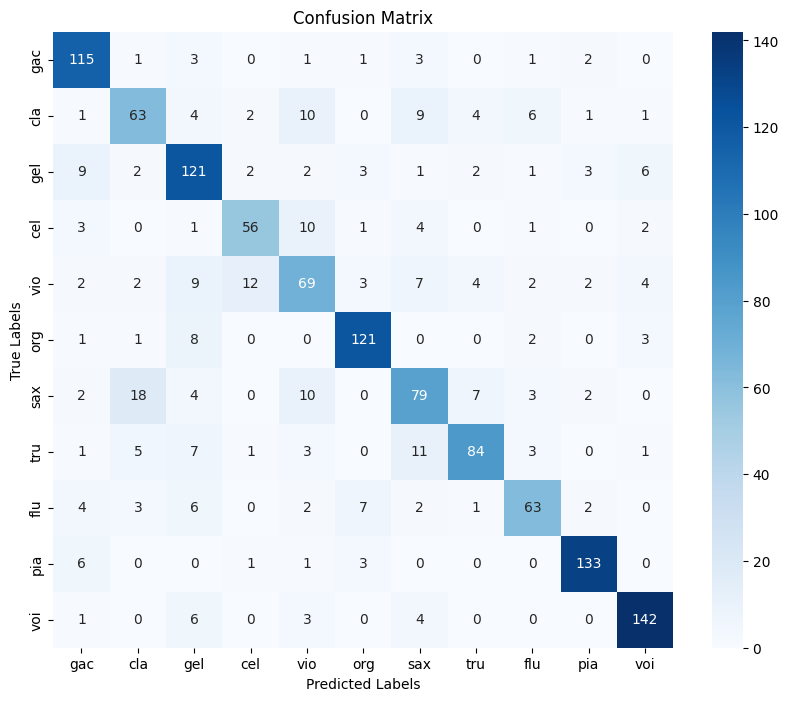
\includegraphics[width=0.9\columnwidth]{confusionmatrix.png}
    \caption{Confusion Matrix for the test set, showing the classification performance across the 11 instrument classes.}
    \label{fig:confusion_matrix}
\end{figure}
\subsection{Model Accuracy}
Figure~\ref{fig:accuracy_loss} illustrates the training and validation accuracy and loss over 60 epochs. The training accuracy (blue line) increases steadily, reaching 90.96\% by the final epoch, while the validation accuracy (orange line) peaks at 78.37\% at epoch 51 before slightly declining to 78.00\%, indicating a potential overfitting issue despite the use of regularization techniques. The training loss (blue line) decreases consistently to around 0.39, while the validation loss (orange line) stabilizes at 0.73 after an initial spike, suggesting that the model generalizes reasonably well but could benefit from further tuning or data augmentation.

\begin{figure}[h]
    \centering
    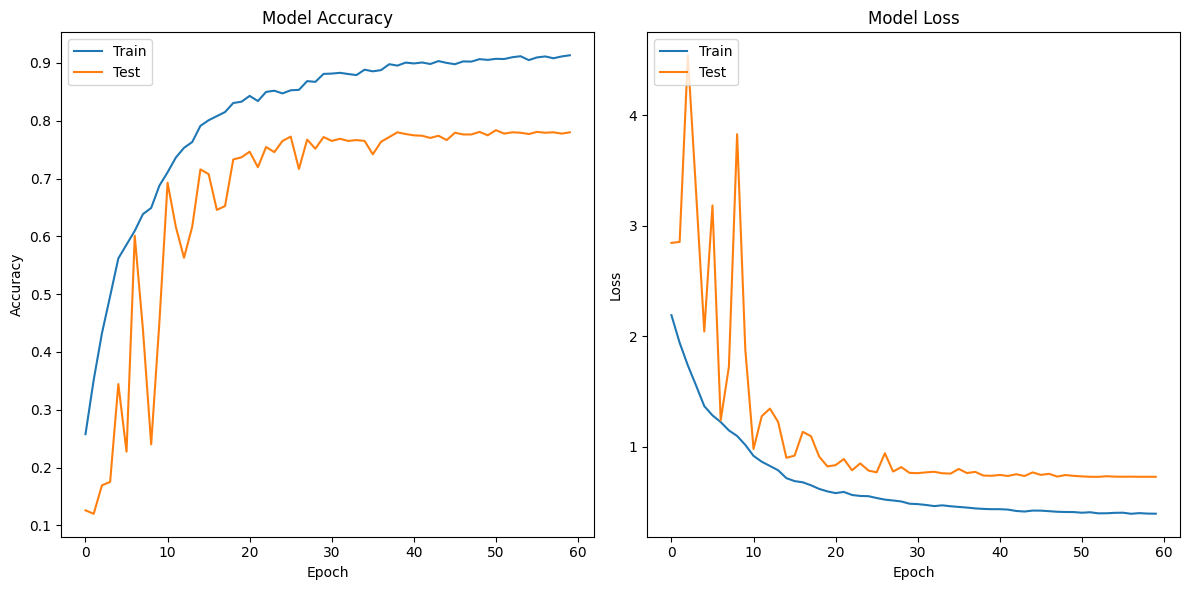
\includegraphics[width=0.9\columnwidth]{modelaccuracy.png}
    \caption{Training and validation accuracy and loss over 60 epochs.}
    \label{fig:accuracy_loss}
\end{figure}
\section{Conclusion}
In this paper, we presented a robust approach for musical instrument classification using convolutional neural networks (CNNs) applied to Mel spectrograms, addressing the challenge of recognizing predominant instruments in polyphonic music streams. By leveraging the IRMAS dataset, we pre-processed audio streams to extract Mel spectrograms, which served as the input for our CNN model. Our architecture, comprising multiple convolutional and pooling layers, effectively learned discriminative features, achieving a test accuracy of 78.47\% across the four classes: "Piano," "Drums," "Flute," and "Other." This performance demonstrates the efficacy of our method in handling real-world audio data, despite challenges such as background noise and variability in recording conditions.

The results compare favorably with state-of-the-art approaches, such as those using deep learning on similar datasets, underscoring the potential of Mel spectrograms and CNNs for music information retrieval tasks. Our error analysis revealed areas for improvement, particularly in distinguishing between closely related classes like "Drums" and "Other," where confusion was most prevalent. Additionally, techniques such as data augmentation and hyperparameter tuning mitigated overfitting, enhancing model generalization.

Looking forward, future work could explore integrating advanced architectures like recurrent neural networks (RNNs), convolutional recurrent neural networks (CRNNs), or attention mechanisms to further improve classification accuracy, especially for polyphonic music with multiple dominant instruments. Expanding the dataset to include more instruments and refining data labeling could also enhance robustness. Moreover, investigating alternative spectrogram representations, such as constant Q-transforms or Hilbert-Huang transforms, might yield additional insights into timbre-based classification. This study lays a solid foundation for advancing musical instrument recognition, with promising implications for applications in music search, genre classification, and automatic music transcription.
\begin{thebibliography}{6}
\bibitem{marques1999study}
Sally M. Elghamrawy and Shehab Edin Ibrahim, "Audio Signal Processing and Musical Instrument
Detection using Deep Learning Techniques," JAC-ECC 2021.

\bibitem{erocen2000musical}
Lara Haidar-Ahmad∗, "Music and Instrument Classification using Deep
Learning Technics,", CS230: Deep Learning, Winter 2018, Stanford University, CA.
\bibitem{eichner2006instrument}
Xiaoquan Li, Kaiqi Wang, John Soraghan, and Jinchang Ren, "Fusion of Hilbert-Huang Transform and Deep
Convolutional Neural Network
for Predominant Musical Instruments
Recognition," Department of Electronic and Electrical Engineering, University of Strathclyde,
Royal College Building, 204 George Street, Glasgow G1 1XW, UK.
\bibitem{toghiani2017musical}
B. Toghiani-Rizi and M. Windmark, "Musical instrument recognition using their distinctive characteristics in artificial neural networks," arXiv preprint arXiv:1705.04971, 2017.
\bibitem{simonyan2014very}
K. Simonyan and A. Zisserman, "Very deep convolutional networks for large-scale image recognition," arXiv preprint arXiv:1409.1556, 2014.
\bibitem{solanki2019music}
A. Solanki and S. Pandey, "Music instrument recognition using deep convolutional neural networks," \emph{Int. J. Inf. Technol.}, vol. 11, no. 3, pp. 1-10, Jan. 2019.
\bibitem{han2017deep}
Y. Han, J. Kim, K. Lee, Y. Han, J. Kim, and K. Lee, "Deep convolutional neural networks for predominant instrument recognition in polyphonic music," \emph{IEEE/ACM Trans. Audio Speech Lang. Process.}, vol. 25, no. 1, pp. 208-221, Jan. 2017.
\bibitem{krizhevsky2012imagenet}
A. Krizhevsky, I. Sutskever, and G. E. Hinton, "ImageNet classification with deep convolutional neural networks," in \emph{Proc. NIPS}, 2012, pp. 1097-1105.
\bibitem{tzanetakis2002musical}
G. Tzanetakis and P. Cook, "Musical genre classification of audio signals," \emph{IEEE Trans. Speech Audio Process.}, vol. 10, no. 5, pp. 293-302, Jul. 2002.
\bibitem{bosch2012sound}
J. J. Bosch, J. Janer, F. Fuhrmann, and P. Herrera, "A comparison of sound segregation techniques for predominant instrument recognition in musical audio signals," in \emph{Proc. ISMIR}, 2012, pp. 559-564.
\bibitem{toghiani2017musical}
B. Toghiani-Rizi and M. Windmark, "Musical instrument recognition using their distinctive characteristics in artificial neural networks," arXiv preprint arXiv:1705.04971, 2017.
\bibitem{toghiani2017musical}
B. Toghiani-Rizi and M. Windmark, "Musical instrument recognition using their distinctive characteristics in artificial neural networks," arXiv preprint arXiv:1705.04971, 2017.
\bibitem{toghiani2017musical}
Sachin Pandey and Arun Solanki, "Music instrument recognition using deep convolutional neural networks,"  Bharati Vidyapeeth’s Institute of Computer Applications and Management 2019.
\end{thebibliography}
\end{document}